%%% The first section of your paper. 

\section{Introduction}

CAD applications are widely popular in Product Design. They aid the design process in presenting easy-to-use ways for defining shapes, attributes, relationships etc. Shapes modeled in CAD can then be used in various downstream applications like drafting, analysis, manufacturing etc. Many commercial CAD applications provide {\em Design-by-Features} approach. {\em Features}, not only carry shape information (geometry, topology) but also embed meta-information based on application's need \cite{Brunetti2003}. {\em Features} also reflect terminologies used in the application thus making them intuitive to use. But this has given rise to various {\em feature-schema} not only in different CAD applications but also in different environments within the same CAD application. Shape that a feature represents could be similar but its {\em feature}-nomenclature, usage, could be different in different environments-applications, e.g. {\em features} like {\em Box}, {\em Pad}, {\em Protrusion}, {\em Extrude}, which appear different, but all could be representing the same shape. This diversity creates problems in learning a new CAD system, interoperability between different CAD applications, and also in development of functionality for downstream applications like, Computer-Aided-Manufacturing (CAM) and Computer-Aided-Engineering (CAE). This is evident in relatively lesser usage of {\em features'} information in the downstream applications, especially CAE.  One of the requirements for leveraging usage of {\em features}, is to come up with a neutral way of defining {\em form features} so that once CAE algorithms are based on them; they can be implemented in variety of CAD-CAE applications. This paper presents such novel formulation of {\em form features} in terms of Spatial Grammars and demonstrates its use to further formulate {\em features} for downstream applications, like {\em Midsurface} for CAE. This approach is exciting as it has potential to address various interoperability and algorithmic issues in variety of CAD based applications.

\section{Related Work}

	Following section explores salient work done so far in the areas relevant to the topic, like, Spatial Grammars, Feature Representation and Midsurface Representation.

\subsection{Spatial Grammars}

Spatial Grammars is a general term which encompasses shape definition Grammars, like Graph Grammars, Shape Grammars, Set Grammars etc. Aim of Spatial Grammars is to bring formalism through terse but expressive definitions, validations and generation of new evolutionary shapes.  Although Spatial Grammars theory seems to have progressed a lot but their practical usage in applications like CAD appears limited, especially in the Mechanical Design domain.

Shape Grammar in a generative approach was formally introduced by Stiny and Gips \cite{Stiny1971} and is primarily used for exploratory, evolutionary design process. It is defined by set of shapes, labels and rules. Its usage in mainstream applications is marred by its complexity of defining and editing the rules.

Hoisl et. al.\cite{Hoisl2009}  proposed a Spatial Grammar based system with implementation in CAD for generative solutions. They used primitives like block, cylinder, cone as initial shapes and proposed use of {\em sweeping} to generate different shapes depending on different profiles and guide curves. Boolean operations were used to build more complex shapes. CAD Grammars proposed by \cite{Deak2006} combined Shape and Graph Grammars to be more useful in Design, Modeling and Manufacturing. They claimed that traditional Shape Grammar could not work well with the CAD primitives and it would be desirable to have such a representation that will work with different CAD systems.

In general there has been limited success to the usage of Spatial Grammars in CAD and in the downstream applications, so far, especially for the purpose of neutral {\em feature} definitions.

\subsection{Feature Representation}

A generally accepted definition of {\em feature} is that  it represents shape as well as functionality significant to a particular product life-cycle phase \cite{Berg2002}. {\em Features} embed application specific high level knowledge and manifest differently as per the context \cite{mandorli1996}. {\em Features} through use of taxonomy, semantics and ontology  bring formalized knowledge representation which can be leveraged to address problems such as interoperability between CAD system and developing downstream applications such as CAE, CAM etc \cite{BidarraBronsvoort2000}, \cite{Tessier2011}, \cite{Ma2013}.

Use of Spatial Grammar to represent {\em form features} is relatively new and is not widely utilized in the commercial CAD applications. This paper attempts to come up with such representation and later uses it to develop a CAE feature, called {\em Midsurface}.


\subsection{Midsuface Representation}

Midsurface is an abstraction of thin-walled portions of a solid into surfaces as part of Model Simplification done for CAE process. It is a surface that lies midway and carries thickness information needed to define 2D shell elements (Figure \ref{figure_Midsurf}). There are various techniques to extract Midsurface mentioned in academic world as well as available in commercial CAD-CAE applications. Predominant among those are Medial Axis Transform (MAT) and Midsurface Abstraction (MA) methods. Survey papers like \cite{Lam1992} and \cite{Attali2004}  have enumerated various approaches used in the Midcurve-Midsurface creation.

	\begin{figure}[h]
	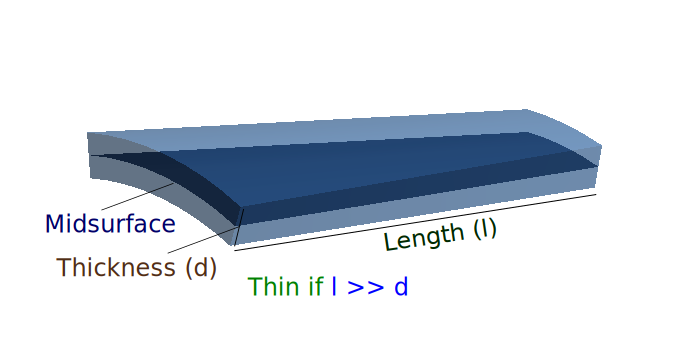
\includegraphics[scale=0.4]{../Common/images//Midsurf.pdf}
	\caption{Midsurface}
	\label{figure_Midsurf}
	\end{figure}

MAT is a locus of the centers of a maximal diameter disc as it rolls around inside the shape. In 2D it is called as 'Midcurve' where as in 3D it is called as 'Midsurface'. Major deficiency of this method is that it creates unnecessary branches and is smaller than the corresponding faces on the original solid. Also, slight change in the base geometry forces re-computation resulting in different MAT than the earlier. 

MA constructs Midsurface by joining individual mid-patches obtained from 'pairs of surfaces'. This approach has benefits over the MAT technique as Midsurface is cleaner and represents parent shape better; but finding pairs in complex shapes is challenging and error prone. 

Most of these approaches are based on the final shape represented typically by Boundary Representation (Brep) solid and do not use feature information\cite{Smit2011}. Midsurface still lacks exact definition, formalism and algorithms to take care of all practical shapes. This paper proposes use of {\em form features} defined in terms of Spatial Grammars in formulating Midsurface.
